\section{Aufgabe 3 - Realisierung eines Logic Analyzers}
\label{sec:aufgabe-3---realisierung-eines-logic-analyzers}

Es ist eine Schaltung zu entwerfen, welche Logikbausteine erkennt.
Da bei zwei Signalen $a$ und $b$ als Eingänge je nach Baustein, bzw.\ Gatter, ein anderes Signal $y$ am Ausgang anliegt, kann ein unbekanntes Gatter analysiert und benannt werden.


\subsection{Materialien}
\label{subsec:a3-materialien}

\begin{table}[h]
    \centering
    \caption{Aufgabe 3 - Verwendete Materialien}
    \label{tab:a3-materialien}
    \begin{tabular}{| l | l | l |}
        \hline
        Bezeichnung & Eigenschaften & Menge \\
        \hline
        Widerstand  & $150\Omega$   & 2     \\
        & Braun - Grün - Braun - Gold & \\
        74HC00 & NAND & 1 \\
        74HC02 & NOR  & 1\\
        74HC08 & AND & 1\\
        74HC32 & OR & 1\\
        74HC86 & XOR  & 1\\
        Mikrocontroller & Arduino Uno R3 & 1 \\
        \hline
    \end{tabular}
\end{table}


\subsection{Vorbereitung}
\label{subsec:a3-vorbereitung}

Zur Vorbereitung dieser Aufgabe, müssen die Wahrheitstabellen der zu untersuchenden Funktionen bekannt sein.
Dafür werden die Tabellen für die verwendeten Funktionen aufgestellt.
Es gilt die Annahme, dass die Funktionen bekannt sind und werden daher nicht näher erklärt.
Eine Erklärung der logischen Funktionen würde über den Umfang dieses Protokolls hinaus gehen.
Die Tabellen können in den Tabellen \ref{tab:wahrheitstabellen-verwendeter-logikfunktionen} angelesen werden.

\begin{table}[ht]
    \centering
    \caption{Wahrheitstabellen verwendeter Logikfunktionen}
    \label{tab:wahrheitstabellen-verwendeter-logikfunktionen}
    \begin{tabular}{| l | l || l |}
        \hline
        & AND & \\
        \hline
        A & B & Y \\
        \hline
        0 & 0 & 0 \\
        0 & 1 & 0 \\
        1 & 0 & 0 \\
        1 & 1 & 1 \\
        \hline
    \end{tabular}
    \quad
    \begin{tabular}{| l | l || l |}
        \hline
        & OR & \\
        \hline
        A & B & Y \\
        \hline
        0 & 0 & 0 \\
        0 & 1 & 1 \\
        1 & 0 & 1 \\
        1 & 1 & 1 \\
        \hline
    \end{tabular}
    \quad
    \begin{tabular}{| l | l || l |}
        \hline
        & NAND & \\
        \hline
        A & B & Y \\
        \hline
        0 & 0 & 1 \\
        0 & 1 & 1 \\
        1 & 0 & 1 \\
        1 & 1 & 0 \\
        \hline
    \end{tabular}
    \quad
    \begin{tabular}{| l | l || l |}
        \hline
        & NOR & \\
        \hline
        A & B & Y \\
        \hline
        0 & 0 & 1 \\
        0 & 1 & 0 \\
        1 & 0 & 0 \\
        1 & 1 & 0 \\
        \hline
    \end{tabular}
    \quad
    \begin{tabular}{| l | l || l |}
        \hline
        & XOR & \\
        \hline
        A & B & Y \\
        \hline
        0 & 0 & 0 \\
        0 & 1 & 1 \\
        1 & 0 & 1 \\
        1 & 1 & 0 \\
        \hline
    \end{tabular}
\end{table}

\newpage

\subsection{Praktikumsaufgabe}
\label{subsec:a3-praktikumsaufgabe2}

Für die Aufgabe wurde nun die in Abbildung \ref{fig:a3-implementiert} gezeigte Schaltung implementiert.
Die Pins 13 und 12 bilden hierfür jeweils die Eingänge für das Logikgatter.
Der Pin 8 liest dann den Ausgang aus.
Die Widerstände von $150\Omega$ wurden verwendet, um die Logikbausteine vor zu hohen Stromflüssen zu schützen.
Mittels des angeschlossenen Multimeters kann der Ausgang manuell ausgelesen werden und das Ergebnis des Programmcodes überprüft werden.

\begin{figure}[ht]
    \centering
    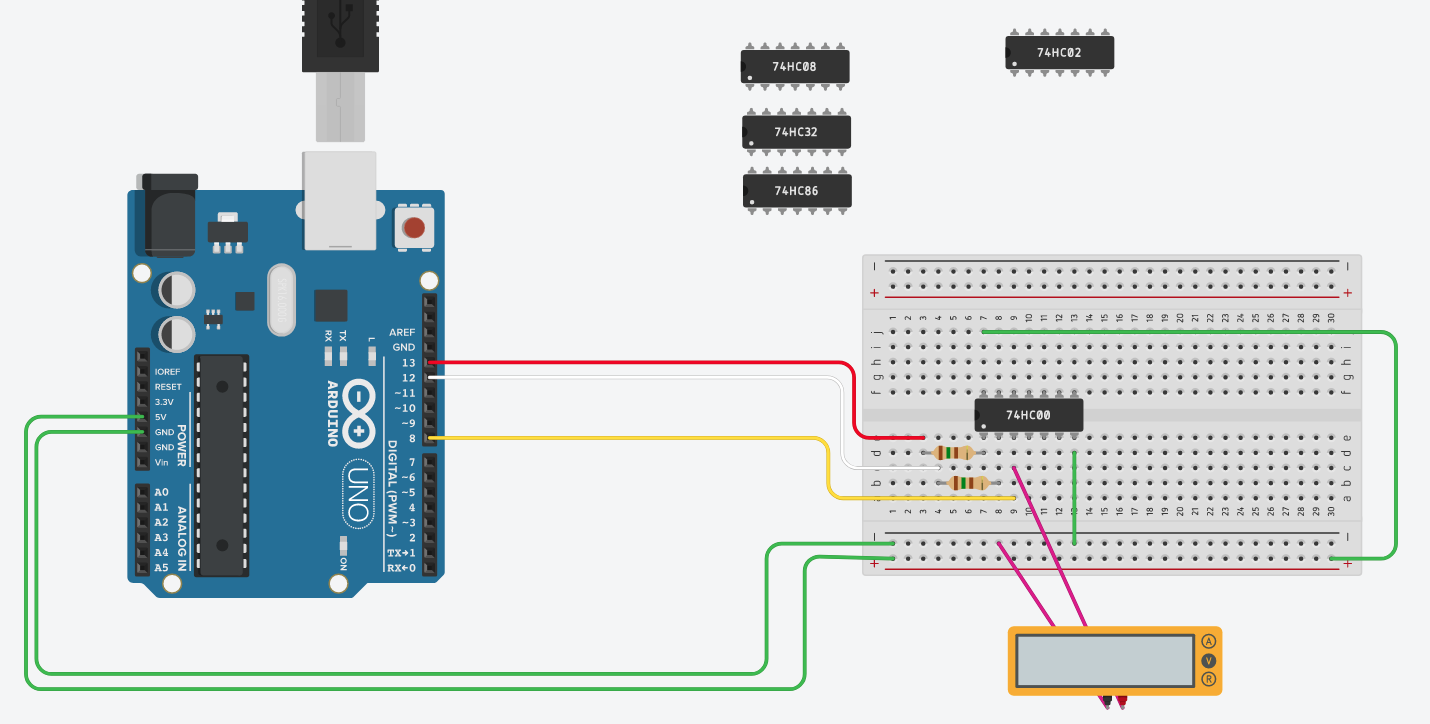
\includegraphics[width=0.9\textwidth]{pictures/a3-praktik.png}
    \caption{Implementierter Stromkreis von Aufgabe 3}
    \label{fig:a3-implementiert}
\end{figure}

Im nachfolgendem Text wird der Programmcode der Aufgabe erläutert.
Einzelne Teile des Codes werden ausgewählt und beschrieben.
Am Ende dieser Sektion befindet sich der vollständige Programmcode.

\begin{lstlisting}[language=C,label={lst:a3-truthtable}, caption={Variable für die Wahrheitstabelle}]
/*
(Input1, Input2) => [Index]
(0, 0) => [0]
(0, 1) => [1]
(1, 0) => [2]
(1, 1) => [3]
*/
bool TRUTH_TABLE[] = { false, false, false, false };
\end{lstlisting}

In Listing \ref{lst:a3-truthtable} wird ein Array angelegt, welches die Ergebnisse der Evaluierung speichert.
Im Kommentar sind die Abbildungen der Eingänge auf den jeweiligen Index zu sehen.
D.h., werden beide Eingänge auf 0, bzw.\ $LOW$, geschalten, so wird das Ergebnis an Index 0 gespeichert.

\begin{lstlisting}[language=C,label={lst:a3-ausführen-des-gatters}, caption={Ausführen der Logikfunktionen}]
digitalWrite(PIN_OUTPUT_1, LOW);
digitalWrite(PIN_OUTPUT_2, LOW);

delay(2000);
TRUTH_TABLE[0] = digitalRead(PIN_INPUT) == HIGH;

digitalWrite(PIN_OUTPUT_1, LOW);
digitalWrite(PIN_OUTPUT_2, HIGH);

delay(2000);
TRUTH_TABLE[1] = digitalRead(PIN_INPUT) == HIGH;

digitalWrite(PIN_OUTPUT_1, HIGH);
digitalWrite(PIN_OUTPUT_2, LOW);

delay(2000);
TRUTH_TABLE[2] = digitalRead(PIN_INPUT) == HIGH;

digitalWrite(PIN_OUTPUT_1, HIGH);
digitalWrite(PIN_OUTPUT_2, HIGH);

delay(2000);
TRUTH_TABLE[3] = digitalRead(PIN_INPUT) == HIGH;
\end{lstlisting}

\newpage

Der Code in Listing \ref{lst:a3-ausführen-des-gatters} setzt nacheinander die Eingänge des Gatters auf die Werte der Wahrheitstabellen.
D.h., es werden beide Eingänge auf 0 gesetzt und das Ergebnis im Array gespeichert.
Danach wird ein Eingang auf 1 und der andere auf 0 gesetzt und das Ergebnis wieder im Array gespeichert, u.s.w..

Zwischen den einzelnen Schaltungen der Eingänge wird mittels Aufruf von $delay(2000)$ zwei Sekunden lang gewartet.
Dieser Aufruf ist dazu da, um ein manuelles Ablesen des Multimeters zu ermöglichen und ist für die korrekte Ausführung des Programms nicht notwendig.

\begin{lstlisting}[language=C,label={lst:a3-aausgabe-der-wahrheitstabelle}, caption={Ausgabe der Wahrheitstabelle}]
Serial.println("");
Serial.println("|---|---|---|");
Serial.println("| a | b | y |");
Serial.println("|---|---|---|");

Serial.print("| 0 | 0 | ");
Serial.print(TRUTH_TABLE[0]);
Serial.println(" |");

Serial.print("| 0 | 1 | ");
Serial.print(TRUTH_TABLE[1]);
Serial.println(" |");

Serial.print("| 1 | 0 | ");
Serial.print(TRUTH_TABLE[2]);
Serial.println(" |");

Serial.print("| 1 | 1 | ");
Serial.print(TRUTH_TABLE[3]);
Serial.println(" |");
Serial.println("|---|---|---|");
Serial.println("");
\end{lstlisting}

Die Ergebnisse die in der Variable aus Listing \ref{lst:a3-truthtable} gespeichert wurden, werden in Listing \ref{lst:a3-aausgabe-der-wahrheitstabelle} ausgegeben.
Diese Ausgabe wird gemacht, um eine manuelle Überprüfung des Ergebnisses machen zu können.
D.h., sie wird gemacht um ein Debuggen des Codes zu ermöglichen, ist aber für eine korrekte Ausführung des Programms nicht notwendig.
Das Programm gibt hier die resultierende Wahrheitstabelle, in der Form einer Tabelle wie in Tabellen \ref{tab:wahrheitstabellen-verwendeter-logikfunktionen} dargestellt, aus.

\newpage

\begin{lstlisting}[language=C,label={lst:a3-evaluierung-der-ergebnisse}, caption={Evaluierung der Ergebnisse}]
if (!TRUTH_TABLE[0]
&& !TRUTH_TABLE[1]
&& !TRUTH_TABLE[2]
&& TRUTH_TABLE[3]) {
    Serial.println("AND - Gate");
} else if (!TRUTH_TABLE[0]
&& TRUTH_TABLE[1]
&& TRUTH_TABLE[2]
&& TRUTH_TABLE[3]) {
    Serial.println("OR - Gate");
} else if (TRUTH_TABLE[0]
&& TRUTH_TABLE[1]
&& TRUTH_TABLE[2]
&& !TRUTH_TABLE[3]) {
    Serial.println("NAND - Gate");
} else if (TRUTH_TABLE[0]
&& !TRUTH_TABLE[1]
&& !TRUTH_TABLE[2]
&& !TRUTH_TABLE[3]) {
    Serial.println("NOR - Gate");
} else if (!TRUTH_TABLE[0]
&& TRUTH_TABLE[1]
&& TRUTH_TABLE[2]
&& !TRUTH_TABLE[3]) {
    Serial.println("XOR - Gate");
} else {
    Serial.println("Unrecognized Gate");
}
\end{lstlisting}

Die Ergebnisse werden in Listing \ref{lst:a3-evaluierung-der-ergebnisse} evaluiert.
Je nachdem welche Ausgaben der Logikbaustein getätigt hat, kann nun die entsprechende Funktion gefunden werden.
Dadurch wird das Ergebnis mit den Ergebnissen aus den Tabellen \ref{tab:wahrheitstabellen-verwendeter-logikfunktionen} verglichen.
Gleichen die Ergebnisse denen der Y-Spalte einer Tabelle, so wurde das jeweilige Gatter erkannt und der Name wird ausgegeben.
Sind die Ergebnisse nicht zuzuordnen, so wird die Meldung "Unrecognized Gate", zu Deutsch "Unbekanntes Gatter", ausgegeben.

\begin{lstlisting}[language=C,label={lst:a3-loop}, caption={Programmschleife}]
void loop()
{
}
\end{lstlisting}

\newpage

Die Programmschleife in Listing \ref{lst:a3-loop} ist leer, da der Code für jedes Logikgatter nur einmal ausgeführt werden muss.
Da für jedes Logikgatter die Schaltung umgebaut werden muss, sprich, es muss das Gatter ausgetauscht werden, ist das Ausführen  des Codes in einer Schleife nicht zielführend.

\begin{lstlisting}[language=C,label={lst:a3-code}, caption={Vollständiger Programmcode der Aufgabe 3}]
const int PIN_OUTPUT_1 = 13;
const int PIN_OUTPUT_2 = 12;
const int PIN_INPUT = 8;

/*
(Input1, Input2) => [Index]
(0, 0) => [0]
(0, 1) => [1]
(1, 0) => [2]
(1, 1) => [3]
*/
bool TRUTH_TABLE[] = { false, false, false, false };

void setup()
{
  Serial.begin(9600);

  pinMode(PIN_OUTPUT_1, OUTPUT);
  pinMode(PIN_OUTPUT_2, OUTPUT);
  pinMode(PIN_INPUT, INPUT);

  digitalWrite(PIN_OUTPUT_1, LOW);
  digitalWrite(PIN_OUTPUT_2, LOW);

  delay(2000);
  TRUTH_TABLE[0] = digitalRead(PIN_INPUT) == HIGH;

  digitalWrite(PIN_OUTPUT_1, LOW);
  digitalWrite(PIN_OUTPUT_2, HIGH);

  delay(2000);
  TRUTH_TABLE[1] = digitalRead(PIN_INPUT) == HIGH;

  digitalWrite(PIN_OUTPUT_1, HIGH);
  digitalWrite(PIN_OUTPUT_2, LOW);

  delay(2000);
  TRUTH_TABLE[2] = digitalRead(PIN_INPUT) == HIGH;

  digitalWrite(PIN_OUTPUT_1, HIGH);
  digitalWrite(PIN_OUTPUT_2, HIGH);

  delay(2000);
  TRUTH_TABLE[3] = digitalRead(PIN_INPUT) == HIGH;

  Serial.println("");
  Serial.println("|---|---|---|");
  Serial.println("| a | b | y |");
  Serial.println("|---|---|---|");

  Serial.print("| 0 | 0 | ");
  Serial.print(TRUTH_TABLE[0]);
  Serial.println(" |");

  Serial.print("| 0 | 1 | ");
  Serial.print(TRUTH_TABLE[1]);
  Serial.println(" |");

  Serial.print("| 1 | 0 | ");
  Serial.print(TRUTH_TABLE[2]);
  Serial.println(" |");

  Serial.print("| 1 | 1 | ");
  Serial.print(TRUTH_TABLE[3]);
  Serial.println(" |");
  Serial.println("|---|---|---|");
  Serial.println("");

  Serial.println("Result: ");

  if (!TRUTH_TABLE[0]
      	&& !TRUTH_TABLE[1]
      	&& !TRUTH_TABLE[2]
      	&& TRUTH_TABLE[3]) {
    Serial.println("AND - Gate");
  } else if (!TRUTH_TABLE[0]
      	&& TRUTH_TABLE[1]
      	&& TRUTH_TABLE[2]
      	&& TRUTH_TABLE[3]) {
    Serial.println("OR - Gate");
  } else if (TRUTH_TABLE[0]
      	&& TRUTH_TABLE[1]
      	&& TRUTH_TABLE[2]
      	&& !TRUTH_TABLE[3]) {
    Serial.println("NAND - Gate");
  } else if (TRUTH_TABLE[0]
      	&& !TRUTH_TABLE[1]
      	&& !TRUTH_TABLE[2]
      	&& !TRUTH_TABLE[3]) {
    Serial.println("NOR - Gate");
  } else if (!TRUTH_TABLE[0]
      	&& TRUTH_TABLE[1]
      	&& TRUTH_TABLE[2]
      	&& !TRUTH_TABLE[3]) {
    Serial.println("XOR - Gate");
  } else {
    Serial.println("Unrecognized Gate");
  }
}

void loop()
{
}
\end{lstlisting}

\subsection{Fehlerdiskussion}
\label{subsec:a3-fehlerdiskussion}

Während des Testens des Programms konnten alle Gatter bis auf das NOR-Gatter nicht erkannt werden.
Der Grund dafür war, dass bei gleicher ausrichtung des NOR-Gatters, die Ein- und Ausgänge vertauscht waren.
D.h., die Reihenfolge der Pins der Bausteine war "Eingange 1 - Eingang 2 - Ausgang", außer am NOR-Gatter.
Hier ist die Reihenfolge "Ausgang - Eingang 1 - Eingang - 2".
Um das NOR-Gatter richtig zu erkennen, muss daher die Schaltung entsprechend angepasst werden.
Da die Schaltung theoretisch ein unbekanntes Gatter erkennen soll, müsste daher die Schaltung geändert werden, wenn das Gatter nicht erkannt wurde.
Wird das Gatter danach immer noch nicht erkannt, handelt es sich tatsächlich um ein unbekanntes Gatter, ansonsten um ein NOR-Gatter.
